\section{Function Optimization}
%what we tried, why we tried it, and why it didn't work
%define prior here
Given the vast state complexity present within MtG, an alternative avenue of research with potentially more useful applications was suggested. The task was to train some agent to be able to, given some black box function $f(\boldsymbol{x})$, find $\underset{\boldsymbol{x}_i}{\text{argmin}} (f(\boldsymbol{x}_i))$. Current methods that are used for such situations either require a very large number of iterations (pattern searching, simplex method) or some form of prior for the expected shape of the function (Bayesian optimisation). So, if an agent could be trained to compute the minima within a small number of steps with no explicit prior, that could be useful in a number of cases.

The particular gains of such an agent would probably be most apparent in situations where there is strong, but unknown, similarity between the functions. This is because the agent, if it is to outperform the all purpose methods, is likely to learn an implicit prior over the functions it is trained on. So if it is trained exclusively on functions of the type that it will be used on, then theoretically it can produce better results for such systems without need to define an explicit prior.

Another interesting result from this experiment would be to see what sort of behaviour the agent learns - how does it balance exploration versus exploitation? Does it attempt to perform newton steps or similar to find the lowest point? This could demonstrate better what types of computation is preferred by neural networks of this type. By getting the agent to occasionally save the output to disk, the set of points explored and the values they returned can be analysed, and the behaviour of the agent better understood as well.


This could be defined as  a Markov decision process, where the action is either to trial some $\boldsymbol{x}_i in f(\boldsymbol{x}_i)$ or stop, the state is set of previous observations of $f(\boldsymbol{x}_i)$ and the reward is: 
\begin{equation*}
r = \begin{cases}
 step penalty&  \text{non-terminal} \\
-Loss(f(\boldsymbol{x}), f(\boldsymbol{x}_{min})) & \text{ terminal}
\end{cases}
\end{equation*}
 $Loss(a,b)$ is some function that is at a minimum when $a = b, \forall a \geq b$ and $step penalty$ is some non-positive constant that encourages the agent to reach a minimum in the smallest number of steps. 
In order to define the problem in such a way that it can learn reasonably and fair comparisons could be done it was decided that it was known (or constrained to be) that the minima would lie within some known finite subspace of $\mathbb{R}^n$. In practice this means that the search space and minima were constrained by $x_i \leq x_{max}$ where $x_{max}$ is some known constant.

%a diagram could help, also use maths. like, less words, more Ms
The reward scheme that simply rewards it for the difference between the final return value and the optimum was chosen not only because of its simplicity, but also because of its independence from the x coordinate checked. Under schemes where the x coordinate needs to be close to the minimum x coordinate, it gets penalised for following optimal behaviour into an unfortunate local minimum. Take the example of a function with two minima, the global one,$M_g$ at $x_{min}$ and a local one $M_l$ at $x_{local}$, where $x_{min}$ and $x_{local}$ are far apart. Further suppose that $f(x_{min_l}) = f(x_{min_g}) + \epsilon$ where $\epsilon$ is small. Suppose the agent explored nearby to both of these minima, and happened to observe a point $\hat x_l$ that is closer  enough to the local minima that $f(\hat x_l) < f(\hat x_g)$, where $\hat x_g$ is the closest point observed to the global minima. This means the agent would return $\hat x_l$ as the minima. Under a reward scheme based on x that would be heavily penalised, due to the large distance in x from the global, despite being entirely logical. So a reward scheme based  purely on $f(x)$ is desirable.

For the experimentation, a series of polynomial functions were defined so that their parameters could be passed as an input, allowing existing neural network training architectures to be used. Each polynomial was defined by randomly choosing a set of roots from within the search space, then producing a series of coefficients by multiplying out
$\int \prod_i (x - r_i) dx$, where $r_i$ is the ith root. Where $\boldsymbol{x}$ has multiple dimensions, in each dimension a separate polynomial is defined this way, so that $f(\boldsymbol{x})  = \sum_i \text{Poly}_i(x_i)$ where $\text{Poly}_i(x)$ is the polynomial function for the ith dimension. Then $f(\boldsymbol{x}$ is evaluated at every combination of roots, and the one with the lowest value is the global minima. The full algorithm is detailed in figure~\ref{alg:functiongen}.

\begin{figure}
\begin{algorithmic}
\State Randomly select  $N_{dim}\times N_{roots}$ values within range [$-x_{max}, x_{max}$] as the roots

\Function {expandTerms}{inds, maxind, numloops, d}
            \If {numloops = 0}
               \State val = 1
                \For {each ind stored in inds}
                    \State$ val \gets val*ind$
                \EndFor
               \State \Return{$val$}
            \Else
                \State $val = 0$
                \For{ i = maxind, numloops, -1}
                    \State inds[numloops] = -roots[i][d]  \Comment{roots correspond to (x - a) terms}
                    \State$ val \gets val $+ expandTerms(inds, i-1,numloops -1, d) 
                \EndFor
                \State \Return{$val$}
            \EndIf
      \EndFunction
        
     \For{ j = 1, ndim}
        \For{ i = 1, nroots}
            \State params[j][i] = loopick(\{\}, nroots, i, j)
        \EndFor
    \EndFor
   \State find min by checking all roots
    
  \State params used to make function of x thus:
  \Function F{coords, params}
    \State out = 0
    \For {i = 1, dim}
         \State res = 1/(npar + 1) 
        \State x = coords[i]
        \For {j = 1, npar} 
              \State res = res * x + (params[i][j] /(npar +1 -j))
	    \EndFor
	   \State out =  out + (res*x)
    \EndFor

    \Return out
\EndFunction
\end{algorithmic}
\caption{algorithm to generate the functions}
\label{alg:functiongen}
\end{figure}

Given the variance of these polynomials, and in particular how much the reward changes with higher orders or dimensions, it was necessary to define a more even comparison between the architectures. One useful statistic was the error rate, defined as the proportion of final values that lay more that 5\% of the average absolute value of the minima away from the global minimum. This indicates how many were ``close enough'' to the target. To further normalize things, two baseline agents were created to give a scale for the rewards to be put on. For simplicity of comparison, the number of steps the agent could take was fixed, and $steppenalty$ was set to 0. The baseline agents were a brute force agent that simply divided the search space into equal blocks and looked across all of these, ignoring the values it received. The reward this equal search agent received was defined as 0 relative reward. The other agent uses pattern search, where it checks a grid around the current best location, moves to the new best if there is one, or reduces the grid size if there isn't. The reward this pattern search agent achieved was set as 1 relative reward.

It was decided that, rather than get the agent to learn how to make the comparisons internally (or potentially learn to interpolate between observed values) that the minimum value observed overall would be worked out externally and fed to the neural network as an additional variable. The idea behind this decision is that this frees up the learning in the network to be devoted to finding the best behaviour for the system, rather than having to additionally use up neurons storing this value and performing the comparison in a potentially harmful manner. This does remove the opportunity for the agent to learn how to guess what the true minimum would be based on its observations, but it was decided that such a behaviour would be extremely prone to over fitting and the gains from it would not be worth the cost in terms of the additional learning overheads. Furthermore such an output would simply learn to return lower numbers under the current reward scheme, which means that the reward would also need to consider the x value of the optimum, which had already been discarded.

\subsection{Recurrent Function Optimisation}
The first design that was attempted was based on the work in Recurrent Models of Visual Attention\cite{RVA}. It used the overall structure shown in figure~\ref{fig:RFOarch} The idea is that the internal state of the recurrent neural network would be able to describe the state so that the feed-forwards network can decide what location to look at next. The network would be trained directly with REINFORCE, so only the rewards are needed, not any critic or similar structure. The final output is the minimum value observed, which is tracked at each function evaluation step, and also passed to the RNN to help describe the state space better, as then it doesn't have to learn to do that as well. The recurrence for the architecture that was designed can be seen in fig~\ref{fig:RFOarch}. On top of that structure, the average reward $b$ was also learned as a parameter of the network so that the variance reduction in REINFORCE could be used. One crucial difference is that, unlike with the visual attention paper \cite{RVA}, there is no classification, so no classification loss to train the RNN with, so it is only being trained by the REINFORCE module. The algorithm used to train it is detailed in figure~\ref{alg:rfo}s

\begin{figure}
\centering
\begin{tikzpicture}[ node distance = 0.8cm, > =  stealth]
\def \shift{0.7}
\def \roundwidth{0.65cm}
%create the nodes and link them with arrows
\node (ht1) [] at (0,0){$h_{t-1}$};
\node (jt) [coordinate, right of =  ht1, xshift = \shift cm] {}
	edge[-](ht1);
\node (It) [rectangle, draw, minimum width = 1cm, above = of jt] {$\text{I}_t$}
	edge[-](jt);
\node (Ft1) [rectangle, draw, fill = black!20, minimum width = 1cm, above = of It] {$f(\boldsymbol{x}_{t-1})$}
	edge[->](It);
\node (mt1) [left of = It, xshift = -\shift cm] {$M_{t-1}$}
	edge [->] (It);
\node (xt1) [left of = Ft1, xshift = -\shift cm] {$\boldsymbol{x}_{t-1}$}
	edge [->] (Ft1);
\node (ht) [rectangle, draw, text width = \roundwidth ,minimum height = 2.5cm, xshift = 0.5cm, right = of jt] {$h_t$}
	edge [<-] (jt);
\node (mt) [above = of ht,  circle, draw, text width =\roundwidth] {$M_t$}
	edge [<-] (It.east);
\node (Lt) [below = of ht, rectangle, minimum width = 1.3cm , draw] {$L_t$}
	edge[<-] (ht);
\node (xt) [below = of Lt, circle, draw, text width =\roundwidth] { $\boldsymbol{x}_{t}$}
	edge [<-] (Lt);
\node (jt) [coordinate, right of =  ht, xshift = 1.4 cm] {}
	edge[-](ht);
\node (It) [rectangle, draw, minimum width = 1cm, above = of jt] {$\text{I}_{t+1}$}
	edge[-](jt);
\node (Ft) [rectangle, draw, fill = black!20, minimum width = 1cm, above = of It] {$f(\boldsymbol{x}_{t})$}
	edge[->](It);
\node (ht) [rectangle, draw, minimum height = 2.5cm, text width =\roundwidth, xshift = 0.5cm, right = of jt] {$h_{t+1}$}
	edge [<-] (jt);
\node (mtp) [above = of ht,  circle, draw, text width =\roundwidth] {$M_{t+1}$}
	edge [<-] (It.east);
\node (Lt) [below = of ht, rectangle, minimum width = 1.3cm , draw] {$L_{t+1}$}
	edge[<-] (ht);
\node (xtp) [below = of Lt, circle, draw,text width =\roundwidth] { $\boldsymbol{x}_{t+1}$}
	edge [<-] (Lt);
\node [right of = ht, xshift = \shift cm] {}
	edge [<-] (ht);
\draw (mt) [->] -> (It.west);
\draw [->, dashed] (xt.east) to[  out =0, in =180] (Ft.west);
\end{tikzpicture}

\caption{Architecture for recurrent function optimisation}
\label{fig:RFOarch}
\end{figure}

\begin{figure}
\centering
\begin{minipage}{.8\textwidth}
\begin{algorithmic}
\State $S(\boldsymbol{O}, \boldsymbol{s}_{i-1}; \theta) \mapsto \boldsymbol{s}_i$
\State $Q(\boldsymbol{s} ;\theta) \mapsto \boldsymbol{x} $
\State $G(\mu,\sigma)$  \Comment{Gaussian Noise}
\State choose some initial $b$ \Comment{Baseline reward}
 \Repeat
 	\State Pick some initial $\boldsymbol{x}_i$
 	\Repeat
 		\State observe $f(\boldsymbol{x}_i)$
 		\If $f(\boldsymbol{x}_i) < f(\hat{\boldsymbol{x}}_{min})$
 			\State$ \hat{\boldsymbol{x}}_{min} \gets \boldsymbol{x}_i$
 		\EndIf
 		\State $\boldsymbol{O}_i = \{f(\boldsymbol{x}_i),\boldsymbol{x}_i, f(\hat{\boldsymbol{x}}_{min}), \hat{\boldsymbol{x}}_{min}\} $
 		\State $s_{i+1} = S(\boldsymbol{O}_i, \boldsymbol{s}_{i}; \theta)$
 		\State $\boldsymbol{x}_{i+1} = G(Q(\boldsymbol{s}_{i+1};\theta),\sigma)$ 
 	\Until{Max steps}
	\State $R = f(\hat{\boldsymbol{x}}_{min}) - f(\boldsymbol{x}_min)$
	\State $b \gets b  + \alpha (R - b)$ \Comment{MSE gradient step for $b = \mathbb{E}[R]$}
	\State $\delta = (R - b) \alpha \nabla_\theta \text{log}(Q(\boldsymbol{s}_{i+1})$
	\State Update $\theta$ in the direction of $\delta$ using backpropagation through time
 \Until{Max epochs}
 \end{algorithmic}
 \end{minipage}
 \caption{Algorithm for running and training the Recurrent Function Optimizer}
 \label{alg:rfo}
\end{figure}

Initially it was very unstable, only wanting to search values at the boundaries of the search space. It seemed to be the case that the internal parameters were exploding to massive values and saturating on every pass. So two normalisation hyper parameters were used - the cutoffNorm and the maxOutNorm. The cutoff norm is the maximum L2 norm of all of the gradients of the parameters for all the layers. If the norm exceeds that value, all the gradients are scaled down by the same amount so that the L2 norm for the gradients equals the cutoffNorm. This prevents exploding gradients within the recurrent elements of the network. The maxOutNorm sets the maximum L2 norm of any one layer of the network. Then, like with the cutoffNorm, if the L2 norm for the layer exceeds the maxOutNorm then all of the parameters of that layer are scaled down by the same amount until their L2 norm is that value. This, like weight decay, allows the network to ``forget'' unhelpful learning and also keeps the outputs bounded. Once both of these were applied the agent began to use much more of the space.

Another important trick that significantly improved performance was normalising the inputs to the network. Particularly in the presence of the above parameters, it is necessary to have every input value to the network to be of the same order of magnitude. However, the range of the output of the function isn't known exactly, and its relative magnitude to itself is very important for working out the minimum. The idea that was hit upon to standardise the outputs was to use an approximate upper bound on the output of the function and divide it by that. Because of how the function was defined, the highest order term of the polynomial always has a coefficient of 1 (as any other function could be scaled to be like that anyway). Furthermore, given that the roots are within known bounds, the agent will never ask for $x$ values above those bounds. So if the output of the function approximator is divided by $x_{max}^{p+1}$, where $p$ is the number of parameters used to define the function, then the vast majority of the outputs should lie within the range [$0 - 1$]. Given that actually the agent spends a lot more time within tighter bounds than those, and the other inputs were in the range [$0- x_{max} $] the output was actually divided by $x^p$. This did result in immediate improvement in performance.

Two different forms for the loss function were tried - $Loss(f(\boldsymbol{x}), f(\boldsymbol{x}_{min})) = log(f(\boldsymbol{x}) - f(\boldsymbol{x}_{min} +1))$ and $Loss(f(\boldsymbol{x}), f(\boldsymbol{x}_{min})) = f(\boldsymbol{x}) - f(\boldsymbol{x}_{min})$. The log form was proposed because it was noted that the linear loss produced potentially very large gradients, and there were concerns about stability. However, given more iterations the linear loss proved to reach good results as well.

One other variation that was attempted to try and improve the results, based on how the agent in the visual attention paper \cite{RVA} was trained, was to calculate what the reward would be at every step, and use the gradient based on these to train the agent instead. The results are labelled everystep below, and generally seemed to do worse. The key difference seems to be that the output is based on the lowest observed value, rather than its current estimate of the truth at each step, so it ended up producing large penalties for what were potentially reasonable exploratory steps, and so producing more nuisance gradients that drove the policy away from optimality.

The exact setup chosen for the experimentation, in terms of number of layers and location of non-linearities, is detailed in figure~\ref{fig:exactsetup}. Each white rectangle is a fully connected layer with size equal to the variable written on it. 
\begin{figure}
\centering
\begin{tikzpicture}[ node distance = 0.6cm, > =  stealth,
layer/.style={ rectangle, draw, minimum width  = 4cm, minimum height = 0.8cm },
NL/.style={ rectangle, draw, minimum width  = 1.7cm, minimum height = 0.8cm, rounded corners },
circ/.style={ circle, draw, text width = 0.65cm },
hv path/.style={to path={-| (\tikztotarget)}},
vh path/.style={to path={|- (\tikztotarget)}}
]
%create the nodes and link them with arrows
\node (x) at (0,0) [circ] { ~~$x$};
\node (fx)[circ, below right = of x, label = 80 : \small{normalised}] {$f(x)$}
	edge [<-] (x);
\node (fxmin) [circ, below right = of fx] {\footnotesize{$\hat x_{min}$}}
	edge [<-] (fx);
\node (inm) [rectangle, minimum width  = 3.5cm, minimum height = 0.8cm, fill = black!20, node distance = 1.8cm, below = of fx] {$\times \frac{1}{x_{max}}$}
	edge [<-] (fx);
\draw (inm.north-|x.south) [<-] to (x);
\draw (inm.north-|fxmin.south) [<-] to (fxmin);

\node (inp) [layer, below = of inm] {input size}
	edge [<-] (inm);
\node (nl1) [NL, below = of inp] {non-linearity}
	edge [<-] (inp);
\node (h) [layer, below = of nl1] {hidden size}
	edge [<-] (nl1);
\coordinate [left = of h] (h1);
\coordinate [below = of h1] (h2);
\node (nl2) [NL, below = of h] {non-linearity}
	edge [<-] (h);
\draw (nl2.210) [out = 230, in = 270, looseness = 1.7] to (h2);
\draw (h2) [out = 90, in = 90, ->, looseness = 1.7] to (h.160);

\node (o1) [layer, below = of nl2] {output size}
	edge [<-] (nl2);
\node (nl3) [NL, below = of o1] {non-linearity}
	edge [<-] (o1);
\node (o2) [layer, below = of nl3] {output size}
	edge [<-] (nl3);
\node (noise) [NL, fill = black!20, below = of o2, label = {[red] right: for exploration}] {gaussian noise}
	edge [<-] (o2);
\node (ht) [NL, below= of noise] {HardTanh}
	edge [<-] (noise);
\node (xmul) [rectangle, fill = black!20, below = of ht] {$\times x_{max}$}
	edge [<-] (ht);
\node (xo) [circ, below = of xmul] {$x_{out}$}
	edge [<-] (xmul);
%bounding box
\node (map)[draw, dashed, red, fit = (xmul) (ht), label = {[red, text width = 4cm] right: mapping [-1 - 1] to the boundaries}] {};
\node (func)[draw, dashed, red, fit = (inp)(nl1)(x)(fx)(fxmin), label = {[red, text width = 4cm] right: function input}] {};
\node (locator)[draw, dashed, red, fit = (o1) (nl3)(o2), label = {[red, text width = 4cm] right: location from internal state}] {};
\node (rnn)[draw, dashed, red, fit = (h) (nl2), label = {[red, text width = 4cm] right: RNN}] {};
\end{tikzpicture}

\caption{Layerwise setup for all of the RFO agents}
\label{fig:exactsetup}
\end{figure}


\subsubsection{Experimental Method}
There were four main experiments performed: a comparison of the impact of number of hidden units in the network to performance, a comparison between using ReLU and HardTanh for the transfer functions and with different reward schemes, a comparison of the agent's performance on higher order polynomials, and a comparison of the agent's performance with functions of different dimensions.

As can be seen in figure~\ref{fig:opt1norm}, the agent's performance on the validation data is noisier than it's performance on the training data, but they do track each other quite closely in general. It can also been clearly seen that the performance on the testing and validation data sets are near identical. Furthermore, although there are important differences in what the data shows, the error rate and the reward show similar enough behaviour that, in the interests of space, for all further graphs only the agent's normalised test reward data will be shown. If the agent performing well, then it would have a normalised reward somewhat larger than 1, indicating that it is performing significantly better than the pattern search agent.


%this bit explains why we only consider the test reward and don't concern ourselves too much with the error rate - it was mostly useful in development
\begin{figure}
\centering

\begin{tikzpicture}[scale = 0.8]
\begin{axis}[
    title={Average reward experienced by RFO agent},
    name = rewplot,
    xlabel={Epoch},
    ylabel={Total Reward},
    legend pos=north west,
    ymajorgrids=true,
    %grid style=dashed,
]
 
\addplot table [ color=blue,mark=none,x = epoch, y=optrew, col sep=comma] {graphs/opt1-full-data.csv};
\addplot table [ color=red,mark=none,x = epoch, y=valrew, col sep=comma] {graphs/opt1-full-data.csv};
    \legend{Training, Validation}
    
\end{axis}

\begin{axis}[
    title={Average Error rate experienced by RFO agent},
    at = (rewplot.right of south east), anchor = left of south west, 
    xlabel={Epoch},
    ylabel={Error Rate (\%)},
    legend pos=south west,
    ymajorgrids=true,
    %grid style=dashed,
]
 
\addplot table [ color=blue,mark=none,x = epoch, y=optER, col sep=comma] {graphs/opt1-full-data.csv};
\addplot table [ color=red,mark=none,x = epoch, y=valER, col sep=comma] {graphs/opt1-full-data.csv};
    \legend{Training, Validation}
    
\end{axis}
\end{tikzpicture}



\begin{tikzpicture}[scale = 0.8]
\begin{axis}[
    title={Normalised reward experienced by RFO agent},
    name = rewplot,
    xlabel={Epoch},
    ylabel={norm. Reward},
    legend pos=south east,
    ymajorgrids=true,
    %grid style=dashed,
]
 
  \draw [color = black] (axis cs: -20,1) to node [very near start, above] {\footnotesize{pattern reward}} (axis cs:300,1);
\addplot  [ color=blue] table [mark=none,x = epoch, y= norm test rew, col sep=comma] {graphs/opt1savingrun.csv};
\addplot  [ color=red] table  [mark=none,x = epoch, y=norm val rew, col sep=comma] {graphs/opt1savingrun.csv};
    \legend{Testing, Validation}
    
\end{axis}

\begin{axis}[
    title={Normalised Error rate experienced by RFO agent},
    at = (rewplot.right of south east), anchor = left of south west, 
    xlabel={Epoch},
    ylabel={norm. Error Rate},
    legend pos=south east,
    ymajorgrids=true,
    %grid style=dashed,
]
 
  \draw [color = black] (axis cs: -15,1) to node [very near start, above] {\footnotesize{pattern error rate}} (axis cs:300,1);
\addplot  [ color=blue] table [mark=none,x = epoch, y=norm test ER, col sep=comma] {graphs/opt1savingrun.csv};
\addplot  [ color=red] table [mark=none,x = epoch, y=norm val er, col sep=comma] {graphs/opt1savingrun.csv};
    \legend{Testing, Validation}
    
\end{axis}
\end{tikzpicture}


\caption{RFO learning behaviour and normalised performance across learning}
\label{fig:opt1norm}
\end{figure}

The implementation of the agent was ran on a single GPU for 250 epochs, and tested on the test data after each epoch. There were  163840 training examples generated and 20480 test examples. To simplify the search space for network sizes, the input and output sizes were always set to half the hidden size. The agent was given a linear reward only at the last step for all the experiments except the one comparing reward schemes.

\subsubsection{RFO Results}
%state the hyperparameters along with the intro for each experiment
\begin{figure}
\centering

\begin{tikzpicture}
\begin{axis}[
    title={Normalised reward experienced by RFO agent for different hidden sizes},
    name = rewplot,
    xlabel={Epoch},
    ylabel={norm. Reward},
    legend pos=south east,
    ymajorgrids=true,
    width = \textwidth,
    height = 0.8\textwidth
    %grid style=dashed,
]
  \draw [color = black] (axis cs: -20,1) to node [very near start, above] {\footnotesize{pattern reward}} (axis cs:300,1);
\addplot [mark=none, color = blue] table [ x = epoch, y= norm test rew, col sep=comma] {graphs/exp1long/opt1tsizeit1.csv};
\addplot [mark=none, color = red] table [ x = epoch, y=norm test rew, col sep=comma] {graphs/exp1long/opt1tsizeit2.csv};
\addplot [ mark=none,color = green] table [x = epoch, y=norm test rew, col sep=comma] {graphs/exp1long/opt1tsizeit3.csv};
%\addplot [mark=none, color = black] table [ x = epoch, y=norm test rew, col sep=comma] {graphs/exp1long/opt1tsizeit4.csv};
%\addplot [mark=none,color = blue, style = dashed]table [ x = epoch, y=norm test rew, col sep=comma] {graphs/exp1long/opt1tsizeit5.csv};
%\addplot [ mark=none, color = red, style = dashed] table [x = epoch, y=norm test rew, col sep=comma] {graphs/exp1long/opt1tsizeit6.csv};
%\addplot [mark=none, color = black, style = dashed] table [ x = epoch, y=norm test rew, col sep=comma] {graphs/exp1long/opt1tsizeit7.csv};
    \legend{16,32, 64, 128, 256, 512, 1024,2048}



    
\end{axis}
\end{tikzpicture}


\caption{Comparison of Agent learning for different hidden sizes}
\label{fig:exp1rfo}
\end{figure}
In figure~\ref{fig:exp1rfo} the test performance for the agent given different hidden sizes is detailed. The transfer function was HardTanh, the agent had 20 steps to find the minimum in, the function was a one dimensional quartic, and the rewards were linear and given at episode termination. Every single network size managed to produced a policy that exceeded the performance of the pattern search agent, though the networks with 128 and 256 hidden neurons produced the highest final reward. As the networks get larger, it takes the agent longer to find the initial jump in performance, which the small networks make within the first epoch or so. This jump is probably the agent learning some initial useful representation of state, which then allows it to learn how to make better decisions. For expediency and peak performance, a hidden size of 128 was chosen to be the norm for other experiments.

\begin{figure}
\centering

\begin{tikzpicture}
\begin{axis}[
    title={Normalised reward for different reward schemes and HardTanh transfer function},
    name = rewplot,
    xlabel={Epoch},
    ylabel={norm. Reward},
    legend pos=south east,
    ymajorgrids=true,
    width = \textwidth,
    height = 0.67\textwidth
    %grid style=dashed,
]
  \draw [color = black] (axis cs: -20,1) to node [very near start, above] {\footnotesize{pattern reward}} (axis cs:300,1);
\addplot [mark=none, color = blue] table [ x = epoch, y= norm test rew, col sep=comma] {graphs/exp1long/opt1tsizeit4.csv};
\addplot [mark=none, color = red] table [ x = epoch, y= norm test rew, col sep=comma] {graphs/exp3/opt1-estepit1.csv};
  \addplot [mark=none, color = black] table [ x = epoch, y= norm test rew, col sep=comma] {graphs/exp3/opt1-logrewit1.csv};
\addplot [mark=none, color = green] table [ x = epoch, y= norm test rew, col sep=comma] {graphs/exp3/opt1-esteplogrewit1.csv};
  \legend{Linear at end, Linear every step, Log reward at end, Log reward every step}
\end{axis}
\end{tikzpicture}

\begin{tikzpicture}
\begin{axis}[
    title={Normalised reward for different reward schemes and ReLU transfer functions},
    name = rewplot,
    xlabel={Epoch},
    ylabel={norm. Reward},
    legend pos=south east,
    ymajorgrids=true,
    width = \textwidth,
    height = 0.67\textwidth
    %grid style=dashed,
]
  \draw [color = black] (axis cs: -20,1) to node [very near start, above] {\footnotesize{pattern reward}} (axis cs:300,1);
  \addplot [mark=none, color = blue] table [ x = epoch, y= norm test rew, col sep=comma] {graphs/exp3/opt1-reluit1.csv};
\addplot [mark=none, color = red] table [ x = epoch, y= norm test rew, col sep=comma] {graphs/exp3/opt1-estepreluit1.csv};
\addplot [mark=none, color = black] table [ x = epoch, y= norm test rew, col sep=comma] {graphs/exp3/opt1-logrewreluit1.csv};
\addplot [mark=none, color = green] table [ x = epoch, y= norm test rew, col sep=comma] {graphs/exp3/opt1-esteplogrewreluit1.csv};
  \legend{Linear at end, Linear every step, Log reward at end, Log reward every step}
\end{axis}
\end{tikzpicture}

\caption{Comparison of Agent learning for different reward schemes and transfer functions}
\label{fig:exp3rfo}
\end{figure}

In figure~\ref{fig:exp3rfo} the agent's performance with different reward schemes and transfer functions is detailed. The hidden size was 128 neurons, the agent had 20 steps to find the minimum in, and the function was a one dimensional quartic.  What is immediately apparent is that, except with a logarithmic reward scheme, the agent is unstable if it uses a ReLU transfer function. This is probably due to the effect noted when the log reward was devised: that large errors produce very large gradients, which would then dominate the learning and harm convergence. This is far more true for ReLU, which passes large positive values unhampered, than with HardTanh, which cuts off both very high and very low values. Even with the log reward, the HardTanh function produced better peak performance, though interestingly less stably. There could be an argument to use logarithmic rewards along with ReLU based on the apparent relative stability here, however it was decided that better peak performance was preferable here. With HardTanh, log rewards produced similar looking performance,with slightly lower peak values. However the comparison isn't quite fair, as with the same improvement in locations the difference in the log rewards will be less than the difference of the linear rewards ($\log b - \log a < b - a, 1 < a < b $). Telling the agent what reward to receive at each step proved counterproductive, probably because it then put a penalty on every action that didn't improve the observed minimum value, which hampers exploration and muddies learning, as it largely rewards the agent for being lucky with the first few values it observed, rather than behaving optimally.

\begin{figure}
\centering

\begin{tikzpicture}
\begin{axis}[
    title={Comparative reward experienced by RFO agent for different order functions},
    name = rewplot,
    xlabel={Epoch},
    xmin = -10,
    ylabel={norm. Reward},
    legend pos=south east,
    ymajorgrids=true,
    width = \textwidth,
    height = 0.67\textwidth
    %grid style=dashed,
]
  \draw [color = blue] (axis cs: -20,1) to node [very near start, above, blue] {\footnotesize{perfect reward}} (axis cs:300,1);
  \draw [color = black] (axis cs: -20,0) to node [very near start, above] {\footnotesize{pattern reward}} (axis cs:300,0);
\addplot [mark=none, color = blue] table [ x = epoch, y= norm test rew, col sep=comma] {graphs/exp2/opt1paramit1.csv};
\addplot [mark=none, color = red] table [ x = epoch, y=norm test rew, col sep=comma] {graphs/exp2/opt1paramit2.csv};
\addplot [ mark=none,color = green] table [x = epoch, y=norm test rew, col sep=comma] {graphs/exp2/opt1paramit3.csv};
\addplot [ mark=none,color = black] table [x = epoch, y=norm test rew, col sep=comma] {graphs/exp2/opt1paramit4.csv};
  \legend{2 minima, 3 minima, 4 minima, 5 minima}
\end{axis}
\end{tikzpicture}


\caption{Comparison of Agent learning for different order polynomials}
\label{fig:exp2parrfo}
\end{figure}

In figure~\ref{fig:exp2parrfo} the agent's performance on polynomials of increasing order is detailed (2 minima - quartic, 3 minima $x^6$ etc). The transfer function was HardTanh, the agent had 20 steps to find the minimum in, the hidden size was 128 neurons, and the rewards were linear and given at episode termination.  The relative performance of evenly searching the whole space compared to a pattern search changed dramatically as the order increased. Because of that, for this experiment a different normalisation was used, which defines the reward on a scale where 0 is the performance of the pattern search agent, and 1 is the perfect result (0 total reward). It should be noted that the agent attained similar results after the first epoch for each test, but as the order increased, the pattern search agent did worse, so the RFO agent did relatively better. The system consistently outperforms the pattern search, arriving to around 0.85 in this normalisation in each case. This means that the agent's absolute performance does decrease as the order increases, but at 15\% of the rate at which pattern search falls off. It should also be noted that for very high order polynomials it is actually quite likely that several of the minima are quite close in value to the global one, improving the chances of the agent attaining a positive reward quickly.


%detail the numbers used in the experiments and explain what the graphs mean - you can do this now

%detail exactly how these experiments were ran. - what was changed, by how much etc.


\subsubsection{Issues and Evaluation}

In figure~\ref{fig:locexp} the points that the agent checks as it moves through one episode are detailed. Notably there seems to be some combination of exploration and exploitation going on, with the agent hanging close to good values it's observed, whilst also choosing to go right across the range of possible values. It isn't performing some form of gradient step or anything else so intuitive, but it does seem to be stepping in direction for some reason. What exactly is going on would probably require detailed analysis of the neurons within this network, but in any case the results are clear enough - this agent attained a normalised score of 1.8 with an error rate of $<$1\%. 

\begin{figure}
\centering

\begin{tikzpicture}
\begin{axis}[
    title={Points explored by the agent},
    name = pointplot,
    xlabel={timestep},
    ylabel={coordinate},
    colorbar,
    colormap/closeto0,
    ymajorgrids=true,
    width = 0.45\textwidth,
    height = 0.4\textwidth
    %grid style=dashed,
]
\addplot [scatter, point meta= explicit, ultra thick] table [ x =step, y = x, col sep = comma, meta = fx] {graphs/dempoints/demopoints1.csv};
\end{axis}
\end{tikzpicture}

\begin{tikzpicture}
\begin{axis}[
    title={Points explored by the agent},
    name = pointplot,
    xlabel={timestep},
    ylabel={coordinate},
    colorbar,
    colormap/closeto0,
    ymajorgrids=true,
    width = 0.45\textwidth,
    height = 0.4\textwidth
    %grid style=dashed,
]
\addplot [scatter, point meta= explicit, ultra thick] table [ x =step, y = x, col sep = comma, meta = fx] {graphs/dempoints/demopoints2.csv};
\end{axis}
\end{tikzpicture}


\begin{tikzpicture}
\begin{axis}[
    title={Points explored by the agent},
    name = pointplot,
    xlabel={timestep},
    ylabel={coordinate},
    colorbar,
    colormap/closeto0,
    ymajorgrids=true,
    width = 0.45\textwidth,
    height = 0.4\textwidth
    %grid style=dashed,
]
\addplot [scatter, point meta= explicit, ultra thick] table [ x =step, y = x, col sep = comma, meta = fx] {graphs/dempoints/demopoints3.csv};
\end{axis}
\end{tikzpicture}

\caption{Points checked by the agent and their return values}
\label{fig:locexp}
\end{figure}

Overall, from the learning charts it can be noted that the learning is far from smooth, and, at least within the limited number of epochs given, not strictly convergent. This will partially be a product of reinforcement learning, but also due to the use of REINFORCE to train a deterministic policy - the method expects every step the agent takes to be stochastic, whilst with these experiments the noise was only added for the training. For all cases where the agent learned anything there are several large jumps in the agents performance, often after a long plateau of similar performance. These jumps are probably due to the agent learning some representational change that allowed it to improve it's behaviour suddenly, as the agent is learning not only how to make good decisions based on the state, but also how to represent this state to itself. These jumps mean that early stopping is not a good method to use with these networks, as important learning may be occurring without immediate change in received reward.

Ideally these jumps could be avoided by starting the agent off in a better area of the search space, and the performance with larger networks would certainly benefit from escaping from more of the local minima that such networks are naturally susceptible to. So whilst the agent's performance so far has been promising, the hope would be to do even better.

\subsection{Apprenticed RFO}

%discuss how fair the number of RL steps given is or otherwise

%Why don't they converge to the pattern reward?

One suggestion to improve the performance, based on the work in Mastering the game of Go with deep neural networks and tree search\cite{alphaGo}, was to train the agent to first replicate ``expert'' output, then further improve the policy using reinforcement learning as before. The idea is that by first moving to a space where it is making good actions already, it would escape local minima and have a more defined manner in which it would learn to define the state space. The first key challenge with this is to choose what sort of agent it should learn from. Initially it was proposed to get it to learn from a simplex agent, but the implementations of simplex agents within the systems constraints were found to be consistently outperformed by the pattern search agent. So it was decided to use the pattern search agent instead. Ideally the agent would be trained by a Bayesian optimiser, but sadly time constraints prevented this from happening.

One possible advantage of this set up for training the agent is that it makes training the agent for an expensive task without a decent model for it a lot easier. Instead of either training the agent directly on the expensive task, which would take a very long time and lots of computation, instead output data from previously used optimisers could be used to train the agent along with some loose approximation based on the data from those, which should reduce how much computational time the agent has to spend on ``live'' examples.

The agent was trained as follows. For each training function the agent produced an output, and in parallel the pattern search agent produced its own output. Mean squared error loss was used to produce the gradient, where the error was defined as the difference between the output of the agent for that step and the pattern searcher. The agent was trained with this for 125 epochs. Then the same networks were trained using reinforcement learning as with the RFo agent for a further 125 epochs.

\subsubsection{Apprenticed RFO results}
The same set of experiments with the same parameters was ran with the apprenticed RFO as with the pure reinforcement learning agent. %compare both how well it does internally, and to RFO
The graphs are normalised in the same way, and the pattern search level is again indicated. Additionally, the step where the apprenticeship was turned off and the agent swapped to reinforcement learning is marked on each chart with a dot at that point.

\begin{figure}
\centering

\begin{tikzpicture}
\begin{axis}[
    title={Normalised reward experienced by Apprenticed RFO agent for different hidden sizes},
    name = rewplot,
    xlabel={Epoch},
    ylabel={norm. Reward},
    legend pos=south east,
    ymajorgrids=true,
    width = \textwidth,
    height = 0.7\textwidth
    %grid style=dashed,
]
  \draw [color = black] (axis cs: -20,1) to node [very near start, above] {\footnotesize{pattern reward}} (axis cs:300,1);
\addplot [mark = *, mark one*=126, color = blue] table [ x = epoch, y= norm test rew, col sep=comma] {graphs/exp1long/opt2tsizeit1.csv};
\addplot [mark = *, mark one*=126, color = red] table [ x = epoch, y= norm test rew, col sep=comma] {graphs/exp1long/opt2tsizeit2.csv};
\addplot [mark = *, mark one*=126, color = brown] table [ x = epoch, y= norm test rew, col sep=comma] {graphs/exp1long/opt2tsizeit3.csv};

    \legend{16, 32, 64}



    
\end{axis}
\end{tikzpicture}


\begin{tikzpicture}
\begin{axis}[
    title={Normalised reward experienced by Apprenticed RFO agent for different hidden sizes},
    name = rewplot2,
    xlabel={Epoch},
    ylabel={norm. Reward},
    legend pos=south east,
    ymajorgrids=true,
    width = \textwidth,
    height = 0.7\textwidth
    %grid style=dashed,
]
  \draw [color = black] (axis cs: -20,1) to node [very near start, above] {\footnotesize{pattern reward}} (axis cs:300,1);
  \addplot [mark = *, mark one*=126, color = green] table [ x = epoch, y= norm test rew, col sep=comma] {graphs/exp1long/opt2tsizeit4.csv};
\addplot [mark = *, mark one*=126, color = blue] table [ x = epoch, y= norm test rew, col sep=comma] {graphs/exp1long/opt2tsizeit5.csv};
\addplot [mark = *, mark one*=126, color = red] table [ x = epoch, y= norm test rew, col sep=comma] {graphs/exp1long/opt2tsizeit6.csv};
\addplot [mark = *, mark one*=126, color = brown] table [ x = epoch, y= norm test rew, col sep=comma] {graphs/exp1long/opt2tsizeit7.csv};
    \legend{128,256, 512, 1024}



    
\end{axis}
\end{tikzpicture}



\caption{Comparison of Apprenticed RFO learning for different hidden sizes}
\label{fig:exp1apprfo}
\end{figure}

Figure~\ref{fig:exp1apprfo} details the normalised reward the apprenticed agent received for different sizes of network. The transfer function was HardTanh, the agent had 20 steps to find the minimum in, the function was a one dimensional quartic, and the rewards were linear and given at episode termination. Of immediate note is that, except for the 16 neuron network, by the end of the apprenticeship every network had converged to a policy that performed at roughly 0 reward, or as well as dividing the search space up evenly. They also all arrived there in very similar manners, as one might expect from a set of sufficiently large networks with regularisation. The response after the reinforcement learning starts is interesting - all networks with 128 or more neurons make this characteristic jump to a policy in region of 2 relative reward before falling away and descending into seemingly chaotic behaviour. The networks with less neurons fail to make such a jump, but also then are less chaotic. Again a network with 128 neurons seems to produce the best result, though less stably.

\begin{figure}
\centering

\begin{tikzpicture}
\begin{axis}[
    title={Normalised reward for different reward schemes and HardTanh transfer function},
    name = rewplot,
    xlabel={Epoch},
    ylabel={norm. Reward},
    legend pos=south east,
    ymajorgrids=true,
    width = \textwidth,
    height = 0.67\textwidth
    %grid style=dashed,
]
  \draw [color = black] (axis cs: -20,1) to node [very near start, above] {\footnotesize{pattern reward}} (axis cs:300,1);
\addplot [mark = *, mark one*=126, color = blue] table [ x = epoch, y= norm test rew, col sep=comma] {graphs/exp1long/opt2tsizeit4.csv};
\addplot [mark = *, mark one*=126, color = red] table [ x = epoch, y= norm test rew, col sep=comma] {graphs/exp3/opt2-estepit1.csv};
  \addplot [mark = *, mark one*=126, color = black] table [ x = epoch, y= norm test rew, col sep=comma] {graphs/exp3/opt2-logrewit1.csv};
\addplot [mark = *, mark one*=126, color = green] table [ x = epoch, y= norm test rew, col sep=comma] {graphs/exp3/opt2-esteplogrewit1.csv};
  \legend{Linear at end, Linear every step, Log reward at end, Log reward every step}
\end{axis}
\end{tikzpicture}

\begin{tikzpicture}
\begin{axis}[
    title={Normalised reward for different reward schemes and ReLU transfer functions},
    name = rewplot,
    xlabel={Epoch},
    ylabel={norm. Reward},
    legend pos=south east,
    ymajorgrids=true,
    width = \textwidth,
    height = 0.67\textwidth
    %grid style=dashed,
]
  \draw [color = black] (axis cs: -20,1) to node [very near start, above] {\footnotesize{pattern reward}} (axis cs:300,1);
  \addplot [mark = *, mark one*=126, color = blue] table [ x = epoch, y= norm test rew, col sep=comma] {graphs/exp3/opt2-reluit1.csv};
\addplot [mark = *, mark one*=126, color = red] table [ x = epoch, y= norm test rew, col sep=comma] {graphs/exp3/opt2-estepreluit1.csv};
\addplot [mark = *, mark one*=126, color = black] table [ x = epoch, y= norm test rew, col sep=comma] {graphs/exp3/opt2-logrewreluit1.csv};
\addplot [mark = *, mark one*=126, color = green] table [ x = epoch, y= norm test rew, col sep=comma] {graphs/exp3/opt2-esteplogrewreluit1.csv};
  \legend{Linear at end, Linear every step, Log reward at end, Log reward every step}
\end{axis}
\end{tikzpicture}

\caption{Comparison of Apprenticed Agent learning for different reward schemes and transfer functions}
\label{fig:exp3app}
\end{figure}

Figure~\ref{fig:exp3app} details the agents performance with different reward schemes and transfer functions. The hidden size was 128 neurons, the agent had 20 steps to find the minimum in, and the function was a one dimensional quartic. Again ReLU without log rewards is a flop, being unstable even in the apprenticed behaviour, though again the log rewards produce the most stable looking output. This may also just be a product of the log rewards being kinder on errors, as can be seen by it's apparent better performance during apprenticeship, even though during apprenticeship the only variable that matters is the transfer function. Here giving a linear reward at every step with HardTanh looks less terrible, perhaps because the agent was already taking sensible initial actions, so the harm that does to initial actions was lessened. In any case, this data shows the key benefit of the apprenticeship - even in set-ups more susceptible to local minima and instability, by starting the reinforcement learning in a better region it stayed in a better region.

\begin{figure}
\centering

\begin{tikzpicture}
\begin{axis}[
    title={Comparative reward experienced by Apprenticed agent for different order functions},
    name = rewplot,
    xlabel={Epoch},
    xmin = -10,
    ylabel={norm. Reward},
    legend pos=south east,
    ymajorgrids=true,
    width = \textwidth,
    height = 0.67\textwidth
    %grid style=dashed,
]
  \draw [color = blue] (axis cs: -20,1) to node [very near start, above, blue] {\footnotesize{perfect reward}} (axis cs:300,1);
  \draw [color = black] (axis cs: -20,0) to node [very near start, above] {\footnotesize{pattern reward}} (axis cs:300,0);
\addplot [mark = *, mark one*=126, color = blue] table [ x = epoch, y= norm test rew, col sep=comma] {graphs/exp2/opt2-paramit1.csv};
\addplot [mark = *, mark one*=126, color = red] table [ x = epoch, y=norm test rew, col sep=comma] {graphs/exp2/opt2-paramit2.csv};
\addplot [ mark = *, mark one*=126,color = green] table [x = epoch, y=norm test rew, col sep=comma] {graphs/exp2/opt2-paramit3.csv};
\addplot [ mark = *, mark one*=126,color = black] table [x = epoch, y=norm test rew, col sep=comma] {graphs/exp2/opt2-paramit4.csv};
  \legend{2 minima, 3 minima, 4 minima, 5 minima}
\end{axis}
\end{tikzpicture}


\caption{Comparison of Apprenticed Agent learning for different order polynomials}
\label{fig:exp2parapp}
\end{figure}

Figure~\ref{fig:exp2parapp} shows how the apprenticed agent performs on polynomials of increasing order. The transfer function was HardTanh, the agent had 20 steps to find the minimum in, the hidden size was 128 neurons, and the rewards were linear and given at episode termination. Again, because the pattern search agent's performance compared to blindly searching the space changes with polynomial order, the score is normalised on a scale where 0 is the pattern search agent's reward and 1 is zero total reward. There is again the characteristic bounce just as it starts reinforcement learning, but for higher order polynomials the agent recovers to a policy better than the pattern search faster and more smoothly, probably due to the plurality of ``good'' minima available.


\subsubsection{Issues and Evaluation}

\begin{figure}
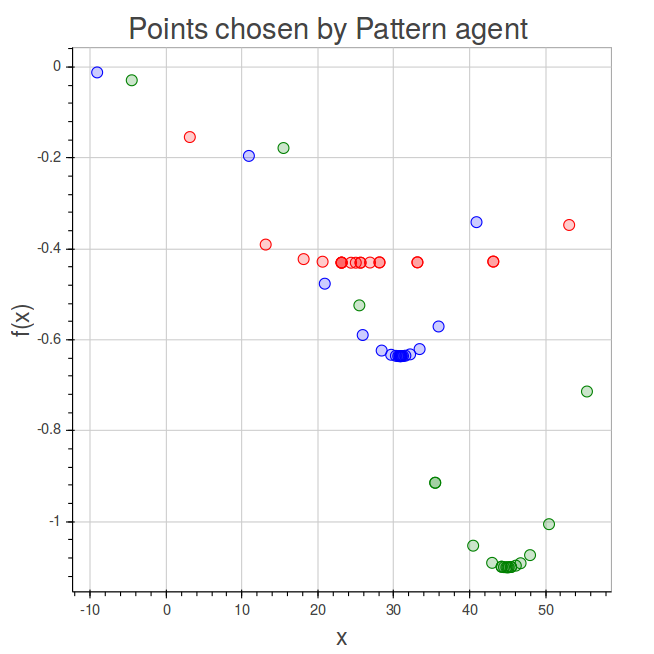
\includegraphics[width = 0.5\textwidth]{pictures/tutorbehav.png} 
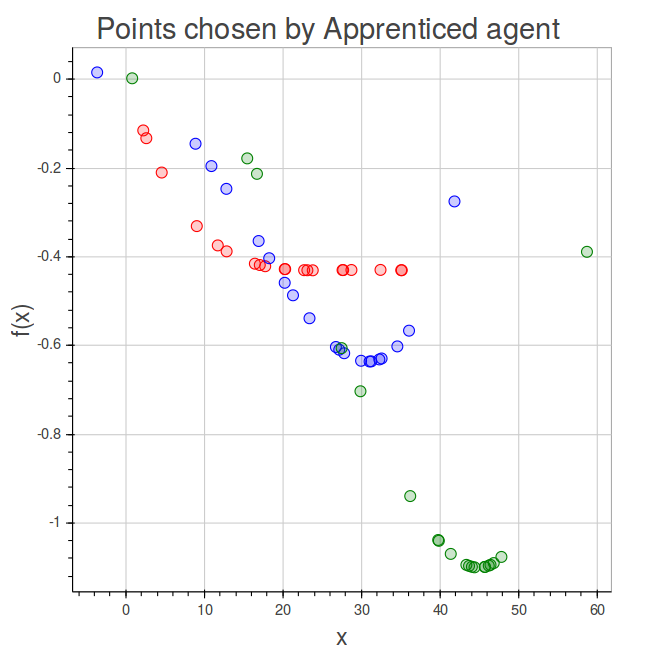
\includegraphics[width = 0.5\textwidth]{pictures/pupilbehav.png}
\caption{Points explored by pattern search agent and apprenticed RFO during apprenticeship}
\label{fig:appbehav}
\end{figure}
One of the key points of interest to look at are that the agent, although it is trained by the pattern search agent, only manages to attain a similar reward to blindly dividing the space into equal chunks. As can be seen in figure~\ref{fig:appbehav}, which is a snapshot taken just before the reinforcement learning starts of three of the episodes, the agent's behaviour is very similar to the pattern search one. In fact, the apprenticed agent gets a normalised error rate pretty close to 1, so it is checking the same minima as the pattern search agent with a similar idea. But unlike the pattern search agent, the apprentice spends a bunch more checks coming down the sides of minima, with a much more even step size, so it doesn't drill down to the absolute minimum value as well. This means that, whilst it makes the same mistakes as the pattern search agent, it additionally gets worse rewards than the pattern search agent does when it is right because it doesn't get as close to the minima. 

The second question is why does it make that bounce as it starts reinforcement learning. The answer is probably that most of it's learning at this point comes from the cases where the pattern search agent does badly, as it does reasonably well on the rest. So initially it learns to explore a bit more so that it can get to those points. It does so, whilst still largely imitating the pattern search agent, and so it gets a reasonable score on most of the cases, resulting in normalised score somewhat above 1. However it is still getting gradients because it isn't making the perfect score. As it applies these changes, it makes some representational change that actually leads to a significant decrease in performance. If left to continue learning for a while, it may reach a different policy, or it may converge to the same policy as the pure RL agent did, depending on the shape of the error surface. However that would take more computational steps than just running the RL, so unless that unknown future policy is even better than just running RL for that long, it doesn't seem worth it.

\begin{table}[hbtp]
\centering
\begin{tabular}{r | cc}
Hidden Size & RFO & Apprenticed \\
\hline
16 & 2.23 & 0.26 \\
32 & 2.47 & 1.89 \\
64 & 2.07 & 1.98\\
128 & 2.66 & 2.40 \\
256 & 2.76 & 2.10 \\
512 & 2.71 & 2.37 \\
1024 & 1.58 & 1.88 \\

\end{tabular}
%\begin{tabular}{c c | cc}
%\multicolumn{2}{c}{Reward scheme}  & & \\
%Function & When  & RFO & Apprenticed \\
%\hline
%Linear & End & 2.66 & 2.40 \\
%Linear & Every step & 0.001 & 2.04 \\
%Log & End & 1.91 & 1.16\\
%Log & Every step & -9.51 & 1.08 \\
%
%\end{tabular}
%These values are scaled so that 0 is the pattern reward and 1 is the best reward possible.
\begin{tabular}{r | cc}
No. minima & RFO & Apprenticed \\
\hline
2 & 0.70 & 0.66 \\
3 & 0.85 &  0.64 \\
4 &0.83  & 0.80 \\
5 & 0.84 & 0.72 \\

\end{tabular}

%need more tables here for the other experiments 

\caption{Best normalised rewards for each of the networks}
\label{tab:compare}

\end{table}

Suppose then that what is desired is for the best agent to be produced in a minimum of steps, and taking the networks from the peak of the bounce is seen as acceptable. The peak normalised rewards each network produced can be seen in table~\ref{tab:compare}. For the same total number of epochs of training, the pure RL agent consistently outperforms the apprenticed agent except with the network with 1024 hidden units. Given that the RL got slower as network size increased, whilst the apprenticed part of the training stayed at the same rate, it can be extrapolated that the apprenticed RFO is better once the RL is that slow or worse. From the shape of the graphs, it would probably be preferable in any implementation using the apprenticeship to end the apprenticeship at 80 epochs rather than 125 so that the subsequent RL has more time to converge.

\subsection{Deterministic RFO}
\label{sec:detrfo}
Given that the environment is both deterministic and non-adversarial, the optimal policy for the agent should be deterministic. So REINFORCE can only ever asymptotically converge to the optimal policy, and given the actual implementation, not even that. So the methods described in Continuous control with deep reinforcement learning\cite{lillicrap2015continuous} ought to be able to produce better performance. A deterministic actor critic agent was created, within the same code structure as the REINFORCE agents, but this one is, in theory, off policy. The total structure of the agent is detailed in figure~\ref{fig:detrfo}. The key additions are the critic networks, which consist of both an RNN that produces an observation of the state, that is the series of value-coordinate pairs so far observed, and the Q-network, which estimates the value of that state.
\begin{figure}
\centering
\begin{tikzpicture}[ node distance =1cm, > =  stealth, hv path/.style={to path={-| (\tikztotarget)}}, vh path/.style={to path={|- (\tikztotarget)}}]
\node (Ft1) [rectangle, draw, fill = black!20, minimum width = 1cm] at (0,0) {$f(\boldsymbol{x}_{n})$};

\node (x) [circle, draw, below right = of Ft1] {\small{$x_{\footnotesize{n+1}}$}};

\node (xn) [circle, draw, node distance = 0.5cm, left = of x] {$x_{n}$};
\draw (xn.north) [->] to (Ft1.south -| xn.north);

\node (RFO) [rectangle, draw, below left = of x, minimum width = 2cm, minimum height = 1.3cm] {RFO}
	edge [->] (x);
\draw (RFO.north -| Ft1.230) [<-] to (Ft1.230);
\draw (RFO.north -| xn.south) [->] to (xn);

\node [rectangle, draw, above right = of Ft1, minimum height = 2cm] (s) {S}
	edge [<-, hv path] (Ft1);
	
\coordinate  [ node distance = 0.4cm, above = of s.85] (s1){}
	edge [bend left = 90] (s.60);
	 
\coordinate  [node distance = 0.4cm, above = of s.95 ] (s2){}
	edge (s1)
	edge [bend right = 90, ->] (s.120); 
	
\node (Q) [rectangle, draw, minimum height = 2cm, right = of s.290] {Q};
\draw (Q.120) [<-, hv path] to (s.325);

\draw (Q.240) [hv path, <-] to (x);

\node (Qv) [right = of Q] {Q($s,x_n$)}
	edge [<-] (Q);
\coordinate [node distance = 4cm, right = of RFO.east](qp)  {};
\draw (qp) [hv path, red] to (Qv);
\draw (qp) [red, ->] to node[near start, below] (drfo){deterministic policy gradient} (RFO);

\coordinate  [above = of Qv, red] (Rp){}
	edge [color = red] (Qv)
	edge [hv path, color = red, ->] (Q);
\draw (Rp) [->, color = red] to node [midway, above, red] {Bellman Update}(s.68);
\node (R) [node distance = 0.5cm, right = of Rp, red] {R}
	edge [color = red] (Rp);
	
\end{tikzpicture}
\caption{Deterministic RFO structure}
\label{fig:detrfo}
\end{figure}

So far the learning with this has been much slower, though more stable than that with REINFORCE, it seems to also get stuck in an unprofitable local minima really easily, as can be seen in figure~\ref{fig:detpolgrad}. It should be noted, however, that it was continuing to improve the policy along that line, just really slowly, which either means its converging into some minima or it's about to jump in a similar manner as with the RFO agent, but at epoch 3000 rather than 30. Given more time, the next step would be to find the hyperparameter set up that gives it the fastest learning rate whilst continuing being stable and running it with the apprenticeship method to get it away from the worse of the local minima.  With the apprenticeship method, the network would be trained by error compared to the tutor whilst the critic learns from the experiences as well so that both are well initialised when it switches to reinforcement learning. Given how slowly it was learning there, the apprenticeship method should significantly save time. However time constraints prevent this from being done within the scope of this project.

\begin{figure}
\centering
\begin{tikzpicture}[scale = 0.8]

\begin{axis}[
    title={Average reward experienced by RFO agent},
    name = rewplot,
    xlabel={Epoch},
    ylabel={Total Reward},
    legend pos=south east,
    ymajorgrids=true,
    %grid style=dashed,
]
 
\addplot [ color=brown]table [mark=none,x = epoch, y=optrew, col sep=comma] {graphs/detpoltestlong.csv};
\addplot [color=red] table [ ,mark=none,x = epoch, y=valrew, col sep=comma] {graphs/detpoltestlong.csv};
    \legend{Training, Validation}
    
\end{axis}

\begin{axis}[
    title={Normalised reward experienced by RFO agent},
     at = (rewplot.right of south east), anchor = left of south west, 
    xlabel={Epoch},
    ylabel={norm. Reward},
    legend pos=south east,
    ymajorgrids=true,
    %grid style=dashed,
]
 
  \draw [color = black] (axis cs: -20,1) to node [very near start, above] {\footnotesize{pattern reward}} (axis cs:300,1);
\addplot [ color=blue] table [mark=none,x = epoch, y= norm test rew, col sep=comma] {graphs/detpoltestlong.csv};
\addplot [ color=red] table [mark=none,x = epoch, y=norm val rew, col sep=comma] {graphs/detpoltestlong.csv};
    \legend{Testing, Validation}
    
\end{axis}


\end{tikzpicture}
\caption{Performance of RFO with deterministic policy gradient}
\label{fig:detpolgrad}
\end{figure}

